\section{Porównanie laserów}
Analizując pomiary dla czterech laserów, które przeprowadziłem, można wyciągnąć następujące wnioski:
\begin{itemize}
\item Sprawność różniczkowa w funkcji zarówno prądu i mocy wejściowej jest większa dla laserów krawędziowych niż dla laserów
VCSEL, co przedstawia wykres na rysunku~\ref{fig:plot_eff}.
\item Prąd progowy dla laserów krawędziowych jest większy od prądu progowego dla laserów VCSEL, co przedstawia wykres
na rysunku~\ref{fig:plot_temp_i_th}.
\item Tabele 5.5--5.8 zawierają porównanie wyznaczonych wartości prądu progowego oraz sprawności różniczkowych z wartościami katalogowymi
firmy Thorlabs. Zmierzone wartości sprawności różniczkowej dla wszystkich laserów zgadzają się z wartościami katalogowymi.
Prąd progowy wyznaczony dla lasera krawędziowego 850\,nm zgadza się z wartością katalogową.
Dla laserów VCSEL wartość prądu progowego nie przekracza wartości maksymalnej podawanej w kartach katalogowych.
Dla lasera krawędziowego 635\,nm wartość maksymalna jest przekroczona niewiele (2\,mA).
\end{itemize}
\newpage
\begin{figure}
\center
  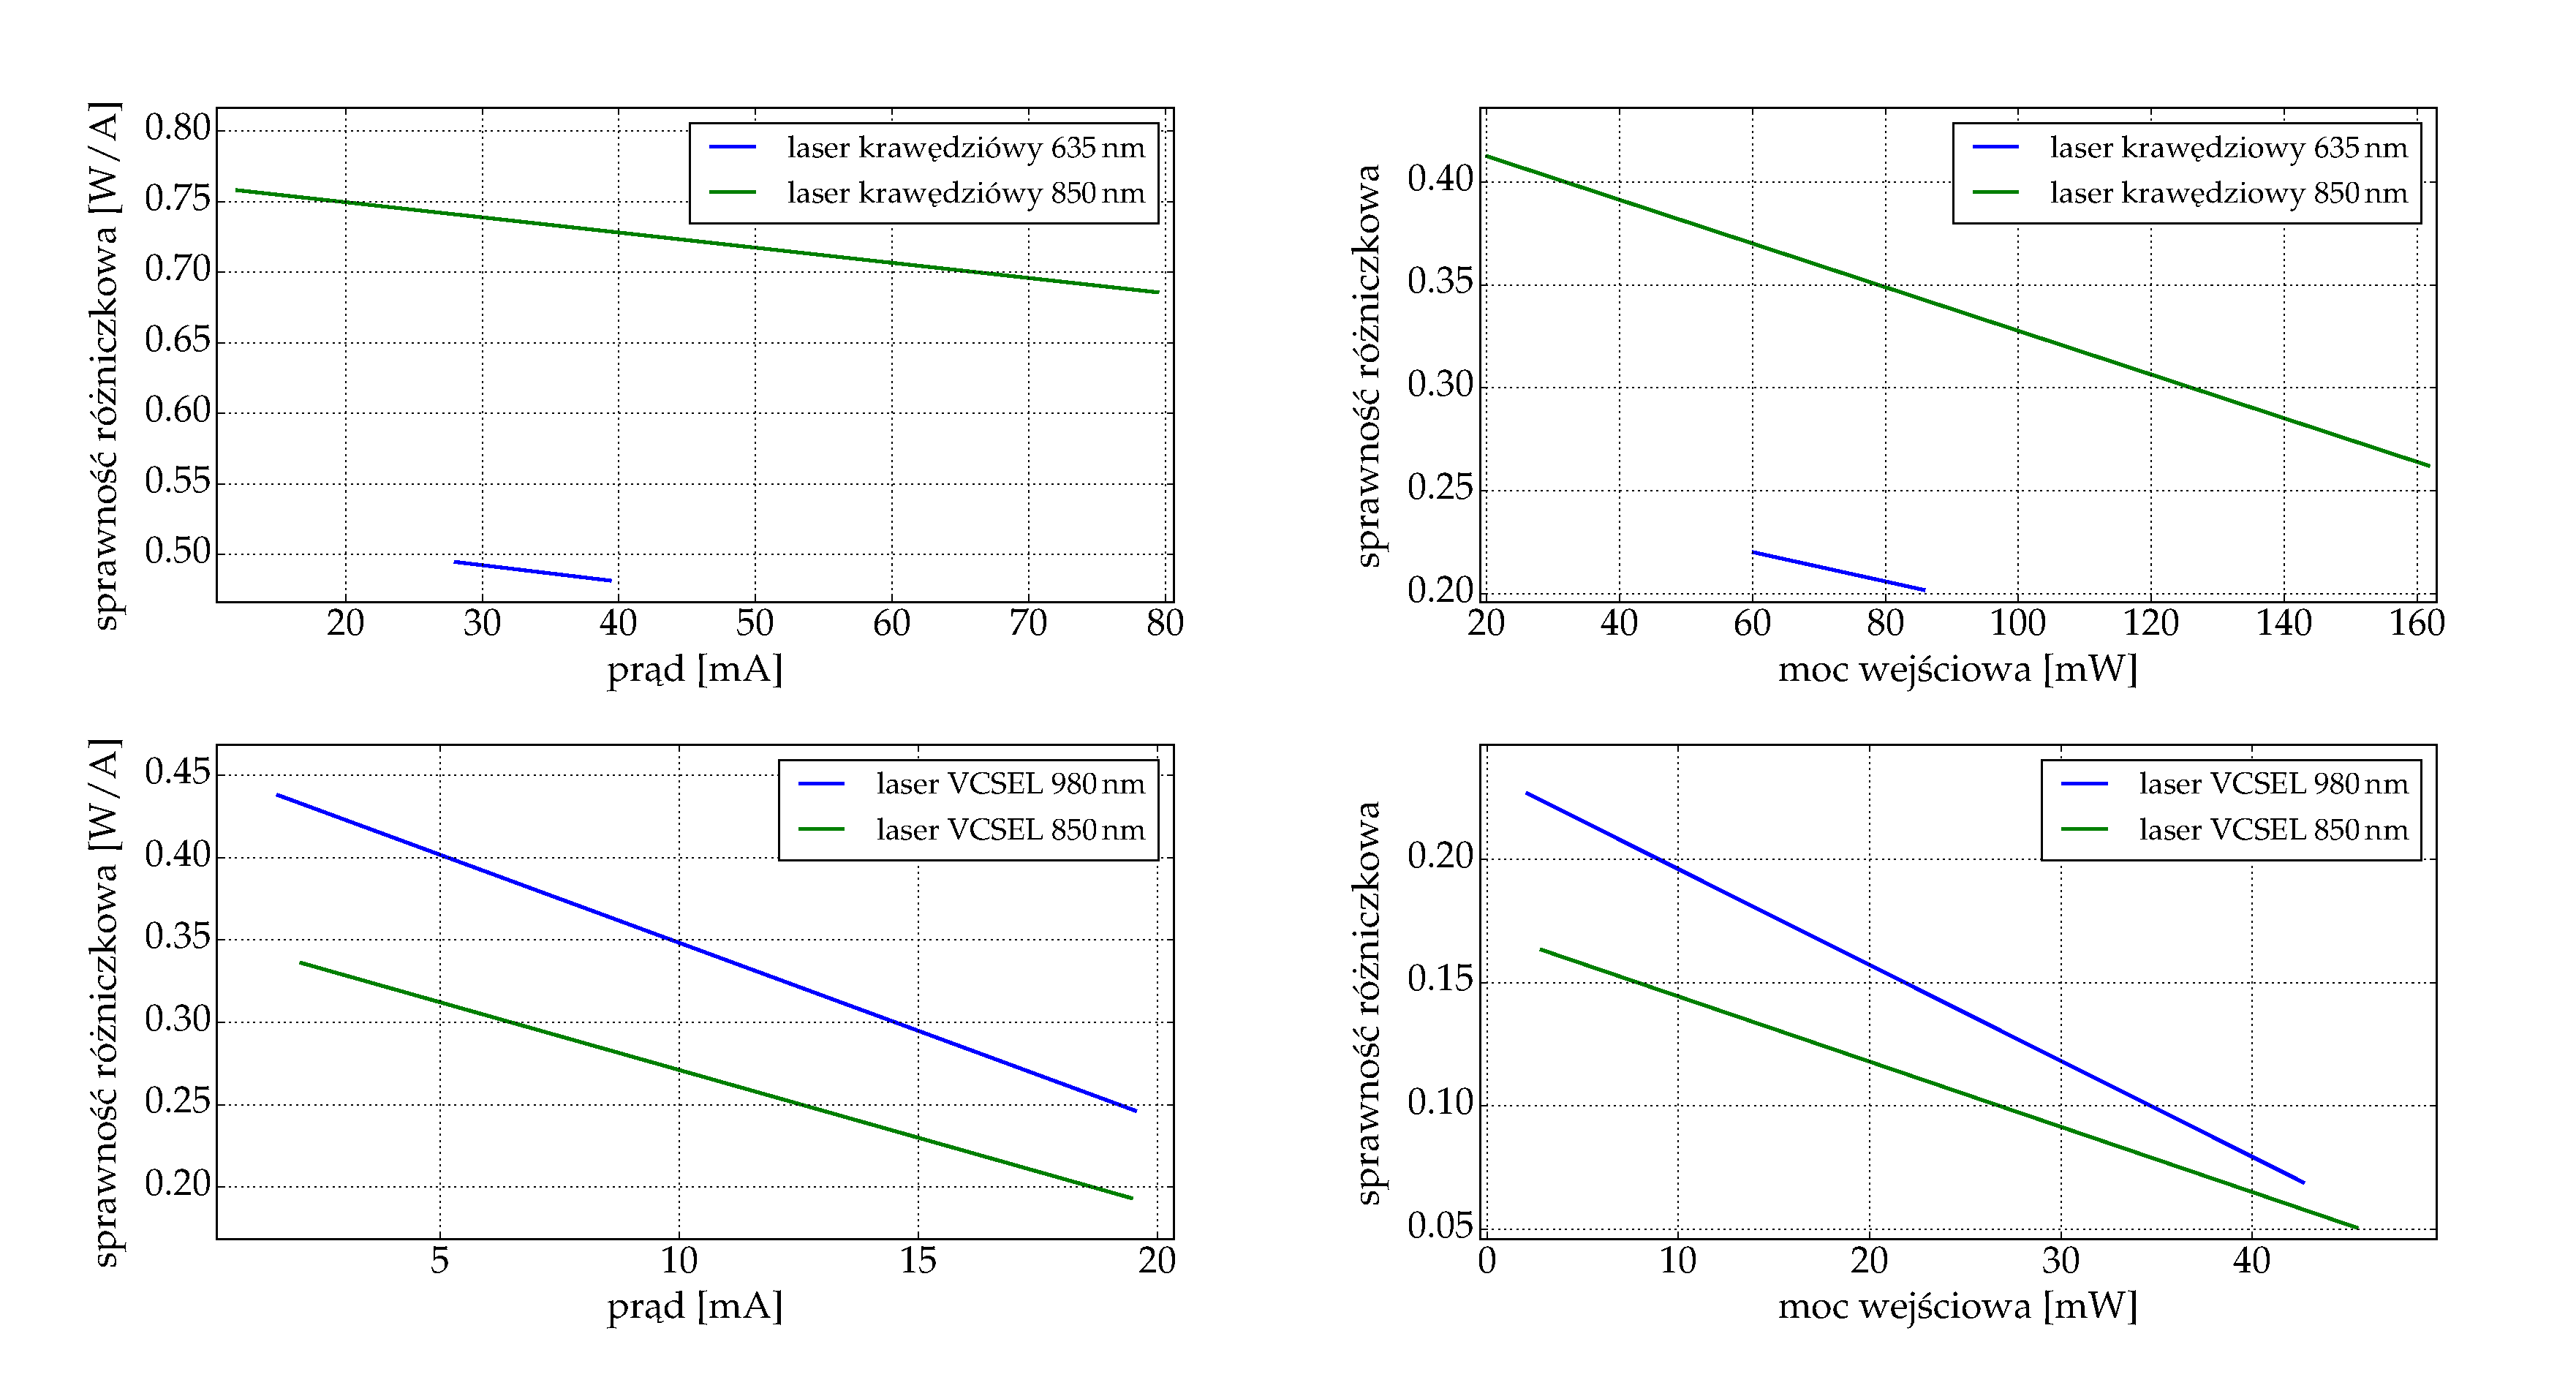
\includegraphics[scale=0.30]{plot_common/plot_eff.eps}
  \caption{Wykres sprawności różniczkowej w funkcji prądu oraz mocy wejściowej w temperaturze 298\,K.}
  \label{fig:plot_eff}
\end{figure}
\begin{figure}[H]
\center
  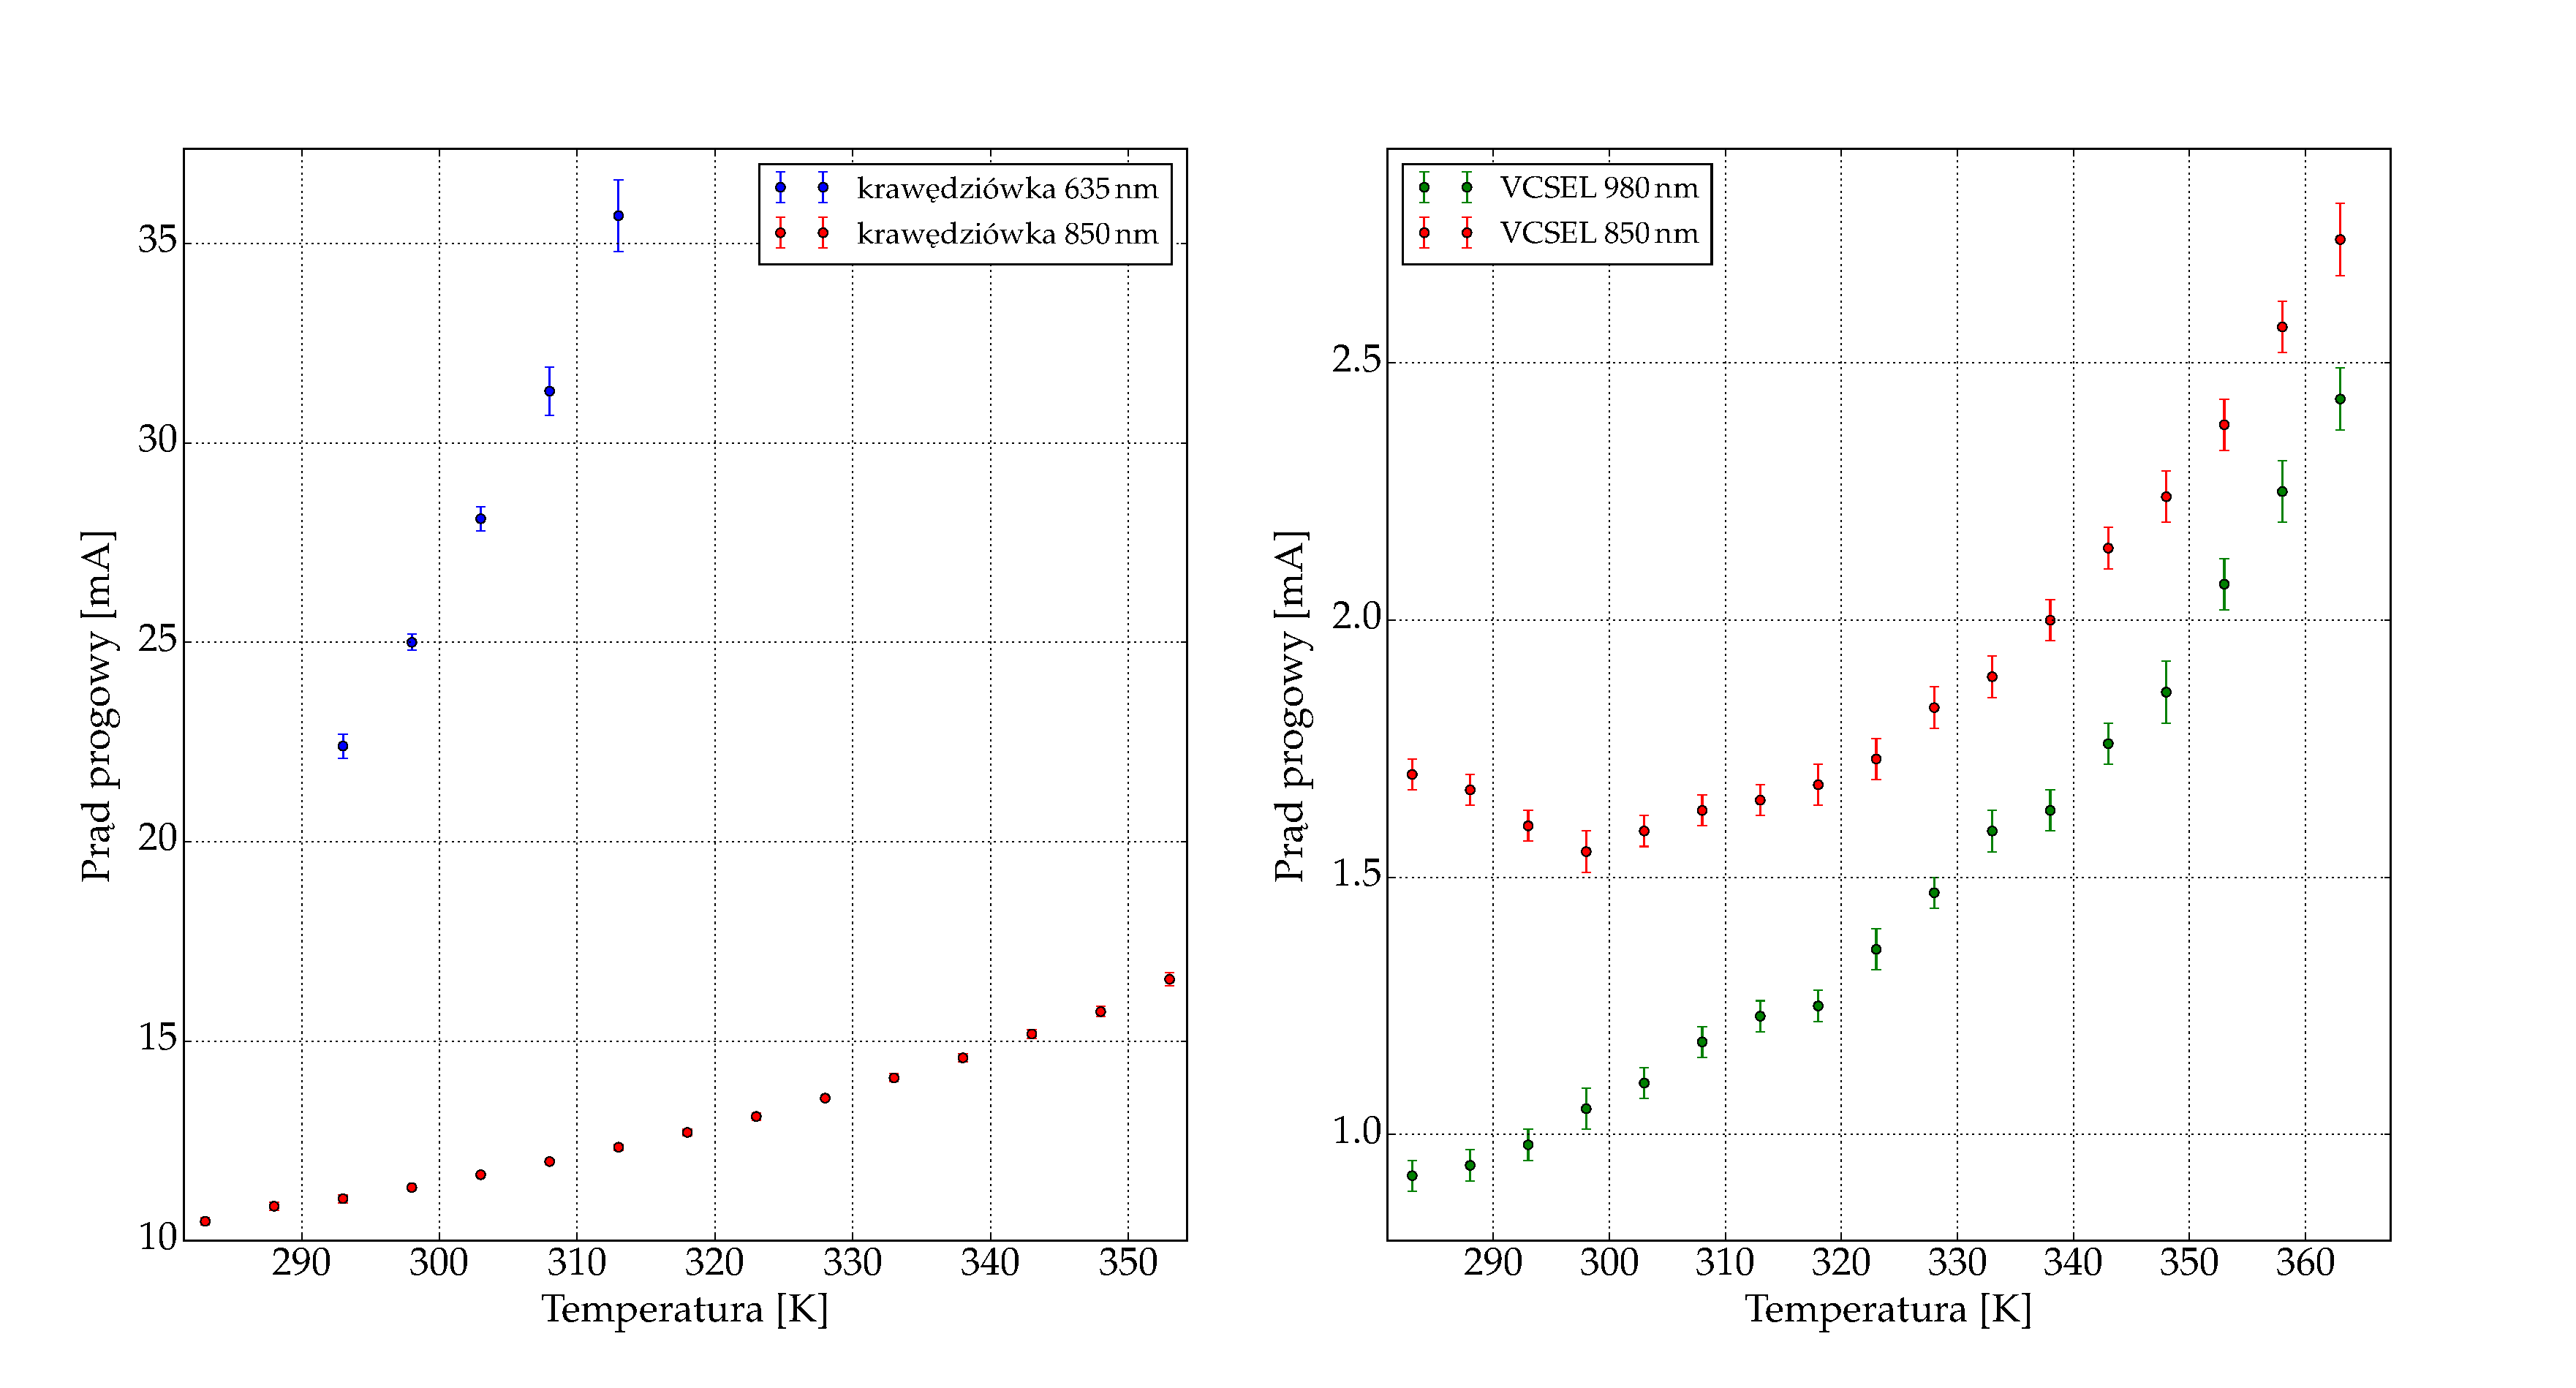
\includegraphics[scale=0.30]{plot_common/plot_temp_i_th.eps}
  \caption{Wykres prądu progowego od temperatury.}
  \label{fig:plot_temp_i_th}
\end{figure}
\newpage
\begin{table}
\begin{center}
\label{tab:tabela1}
\caption{Porównanie wyznaczonych wartości  prądu progowego oraz sprawności różniczkowej z kartą katologową~\cite{spec_vcsel_850}
 w temperaturze 298\,K dla lasera VCSEL 850\,nm. }
\begin{adjustbox}{max width=\textwidth}
\begin{tabular}{ | C{3.5cm}|  C{1.5cm} | C{1.5cm} | C{1.5cm}| C{3.5cm}|}
\hline
           &   Min  & typowy & Max   & wyznaczony        \\ \hline
Prąd progowy [mA] &  --    &  2.2    & 3    & 1.55 $\pm$ 0.04  \\ \hline
sprawność [W/A]  przy $I$ = 8\,mA   &  0.12   &  0.32   & 0.4   & $0.28\pm 0.01$      \\ \hline
\end{tabular}
\end{adjustbox}
\end{center}
\end{table}

\begin{table}
\begin{center}
\label{tab:tabela2}
\caption{Porównanie wyznaczonych wartości prądu progowego oraz sprawności różniczkowej z kartą katologową~\cite{spec_vcsel_980}
 w temperaturze 298\,K dla lasera VCSEL 980\,nm. }
 \begin{adjustbox}{max width=\textwidth}
\begin{tabular}{ | C{3.5cm}|  C{1.5cm} | C{1.5cm} | C{1.5cm}| C{3.5cm}|}
\hline
       &   Min  & typowy & Max   & wyznaczony        \\ \hline
Prąd progowy [mA] &  --    &  2.2    & 3    & 1.05 $\pm$ 0.04  \\ \hline
sprawność [W/A]  przy $I$ = 8\,mA   &  0.12   &  0.32   & 0.4   & $0.37 \pm 0.01$     \\ \hline
\end{tabular}
\end{adjustbox}
\end{center}
\end{table}

\begin{table}
\begin{center}
\label{tab:tabela3}
\caption{Porównanie wyznaczonych wartości prądu progowego oraz sprawności różniczkowej z kartą katologową~\cite{spec_edge_850}
 w temperaturze 298\,K dla lasera krawędziowego 850\,nm. }
\begin{adjustbox}{max width=\textwidth}
\begin{tabular}{ | C{3.5cm}|  C{1.5cm} | C{1.5cm} | C{1.5cm}| C{3.5cm}|}
\hline
         &   Min  & typowy & Max   & wyznaczony        \\ \hline
Prąd progowy [mA] &  10    &  25    & 40    & 11.33 $\pm$ 0.05  \\ \hline
sprawność [W/A]     &  0.3   &  0.5   & 0.7   & $0.5 \pm 0.1$     \\ \hline
\end{tabular}
\end{adjustbox}
\end{center}
\end{table}
\begin{table}
\begin{center}
\label{tab:tabela4}
\caption{Porównanie wyznaczonych wartości prądu progowego oraz sprawności różniczkowej z kartą katologową~\cite{spec_edge_635}
 w temperaturze 298\,K dla lasera krawędziowego 635\,nm. }
\begin{adjustbox}{max width=\textwidth}
\begin{tabular}{ | C{3.5cm}|  C{1.5cm} | C{1.5cm} | C{1.5cm}| C{3.5cm}|}
\hline
        &   Min  & typowy & Max   & wyznaczony        \\ \hline
Prąd progowy [mA] &  --    &  16    & 26    & 27.9 $\pm$ 0.3  \\ \hline
sprawność [W/A]      &  0.4   &  0.6   & 1  &  $0.8 \pm 0.1$       \\ \hline
\end{tabular}
\end{adjustbox}
\end{center}
\end{table}

